\chapter{Implementierung und Design}
\label{sec:implementation}
In diesem Kapitel der Arbeit wird die Implementierung auf Basis der aufgestellten Anforderungen in Kapitel \ref{sec:requirements} betrachtet. Die Verzeichnisstruktur, auf welche in den folgenden Kapiteln eingegangen wird, ist als Baumstruktur mit Abbildung \ref{fig:dirstructure} gegeben. Da die allgemeine Architektur mithilfe der Containervirtualisierung über Docker aufgebaut ist, wird zunächst dieser Aspekt erläutert. Im Anschluss findet jeweils eine Unterscheidung zwischen der Architektur für das Front-End und das Back-End statt.
\begin{marginfigure}
    \centering
    \begin{adjustbox}{width=\textwidth}
        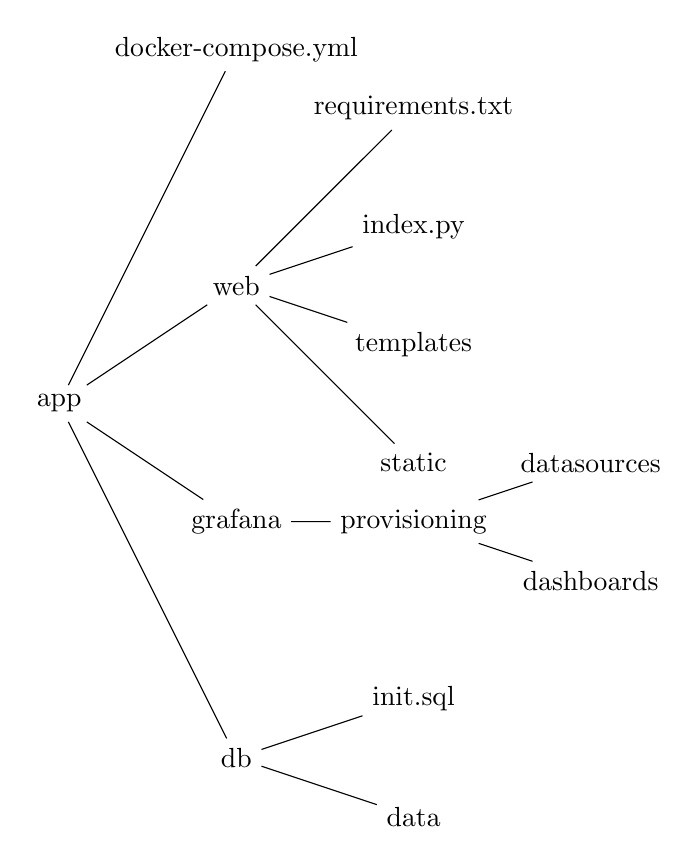
\begin{tikzpicture}[
                grow=right,
                scale=1.5,
                level 1/.style={sibling distance=2cm},
                level 2/.style={sibling distance=1cm}
            ]
            \node{app}
            child { node {db}
                    child { node {data}}
                    child { node {init.sql}}}
            child { node {grafana}
                    child { node {provisioning}
                            child { node {dashboards}}
                            child { node {datasources}}
                        }
                }
            child { node {web}
                    child { node {static}}
                    child { node {templates}}
                    child { node {index.py}}
                    child { node {requirements.txt}}
                }
            child { node {docker-compose.yml}};
        \end{tikzpicture}
    \end{adjustbox}
    \caption{Die Verzeichnisstruktur der Applikation}
    \label{fig:dirstructure}
\end{marginfigure}

\section{Containervirtualisierung mit Docker}
Aufgrund der Tatsache, dass ein privater Entwickler ein Produktivsystem mit mehreren Komponenten simulieren muss, hat sich der Einsatz Dockers als sinnvoll erwiesen. Docker ist eine Open-Source-Software, die es ermöglicht, Anwendungen mithilfe von Containervirtualisierung zu isolieren. Dabei wird die Anwendung in einem Container ausgeführt, der alle Abhängigkeiten enthält, die für die Ausführung der Anwendung erforderlich sind. Die Container sind dabei leichtgewichtiger als virtuelle Maschinen, da sie den Kernel des Host-Betriebssystems nutzen\sidenote{\url{https://www.docker.com/resources/what-container/}}. Für diese Arbeit sind drei Anwendungen notwendig: eine Python-Flask Instanz für einen Webserver (Port 5000), eine PostgreSQL-Instanz für die Datenbank (Port 5432) und eine Grafana-Instanz (Port 3000) für die Verarbeitung und Visualisierung der Daten aus der Datenbank. Diese drei Anwendungen werden jeweils in einem eigenen Container ausgeführt und einem Netzwerk zugewiesen, um eine Kommunikation zwischen den Containern zu ermöglichen (vgl. Abbildung TODO ARCHITEKTUR FÜR DOCKER HIER EINFÜGEN)

\section{Architektur für das Front-End}
Das Front-End der Applikation ist mit dem Web-Framework Python-Flask\sidenote{\url{https://flask.palletsprojects.com/}} und den daraus resultierenden Komponenten umgesetzt. Die Wahl, welche Programmiersprache zur Implementierung des Werkzeugs zum Einsatz kommen soll, fiel auf Python\sidenote{\url{https://www.python.org/}}, da es sich um eine leichtgewichtige und einfach zu erlernende Sprache handelt. Zudem ist Python eine der beliebtesten Programmiersprachen, wird von vielen Entwicklern und bietet daher eine umfangreiche Dokumentation zum Umsetzen der individuellen Anforderungen. 

\section{Architektur für das Back-End}